\documentclass[12pt,letter]{article}


\usepackage{nicefrac,amsmath}
\usepackage[english]{babel}
\usepackage{helvet}
\usepackage{enumerate}
\usepackage{parskip}
%\usepackage{apacite}
\usepackage[english]{babel}
\usepackage{booktabs}
\usepackage[top=1in, bottom=1in, left=1in, right=1in]{geometry}
\usepackage{graphicx}
\usepackage{subfigure}
\usepackage{url}
\usepackage{hyperref}
\usepackage{physics}
\usepackage{cancel}
\usepackage{gensymb}
\usepackage{bbm}
\usepackage{dsfont}
\usepackage{mathtools}
\usepackage{appendix}
\usepackage{etoolbox}

\usepackage{amsfonts}

% Inserts \clearpage before \begin{appendices}
\BeforeBeginEnvironment{appendices}{\clearpage}

\usepackage{algpseudocode}
\usepackage{algorithm}


\usepackage[usenames,dvipsnames]{color}
 \usepackage{listings}
 \definecolor{Brown}{cmyk}{0,0.81,1,0.60}
 \definecolor{OliveGreen}{cmyk}{0.64,0,0.95,0.40}
 \definecolor{CadetBlue}{cmyk}{0.62,0.57,0.23,0}



 \lstset{language=python,
 basicstyle=\small,
 frame=single,
 keywordstyle=\ttfamily\color{OliveGreen}\bfseries,
 identifierstyle=\ttfamily\color{CadetBlue}\bfseries, 
 commentstyle=\color{Brown}\ttfamily,
 stringstyle=\ttfamily\color{red},
 showstringspaces=false}


\newcommand{\argmax}[1]{\underset{#1}{\operatorname{arg}\,\operatorname{max}}\;}
\newcommand{\argmin}[1]{\underset{#1}{\operatorname{arg}\,\operatorname{min}}\;}



%\usepackage{cmbright}
\usepackage[T1]{fontenc}

\usepackage{xcolor}
\usepackage{mdframed}



\setlength{\parskip}{12pt} % 1ex plus 0.5ex minus 0.2ex}

%\renewcommand{\familydefault}{\sfdefault}

\setlength{\parindent}{0cm}
\renewcommand{\baselinestretch}{1.2}

\title{{\bf Optimization using numerical libraries} }


\date{}
\begin{document}
\maketitle
\vspace{-1.0in}

%{\small 
%\tableofcontents
%\listoffigures
%\listofalgorithms
%}

%\newpage



\section{Overview}
\vspace{12pt}
    \begin{mdframed}[backgroundcolor=blue!20] 
        {\bf Question}: Why do we calculate derivatives analytically if computers can calculate them numerically?
    \end{mdframed}
    
One answer to the above question is that numerical-optimization methods produce faster and more precise results when we provide them with the analytical derivative (or gradient, or Jacobian) of the objective function.  This point is discussed further in these notes. 

Analytically, the derivative of a scalar function $f$  of a single variable $x$ is given by: 
\begin{align}
        \dv{f}{x} = \lim_{\Delta x \rightarrow 0}\frac{\Delta f}{\Delta x} = \lim_{\Delta x \rightarrow 0}\frac{f\left(x+\Delta x\right) - f\left(x\right)}{\Delta x}.
	\label{dfx}
\end{align}	
Depending on the type of function, the derivative receives different names such as {\em gradient} and {\em Jacobian}.

\section{Optimization problems}

In many applications, we need to calculate derivatives of functions (e.g., solving optimization problems). In fact, the derivative equations (i.e., in analytical form) may be passed as an input parameter to optimization functions from numerical libraries. While these library functions can calculate the required derivatives numerically, they solve optimization problems more efficiently (and more accurately) if the analytical derivatives are supplied (i.e., user-supplied gradients).


 For example, consider the problem of finding the minimum of the Rosenbrock function\footnote{\url{https://en.wikipedia.org/wiki/Rosenbrock_function}} (Figure \ref{fig_rosenbrock}): 
\begin{align}
f(x,y) = (a-x)^2 + b(y-x^2)^2.
\label{rosenbrock}
\end{align}
\begin{figure}[H]
	\begin{center}
		{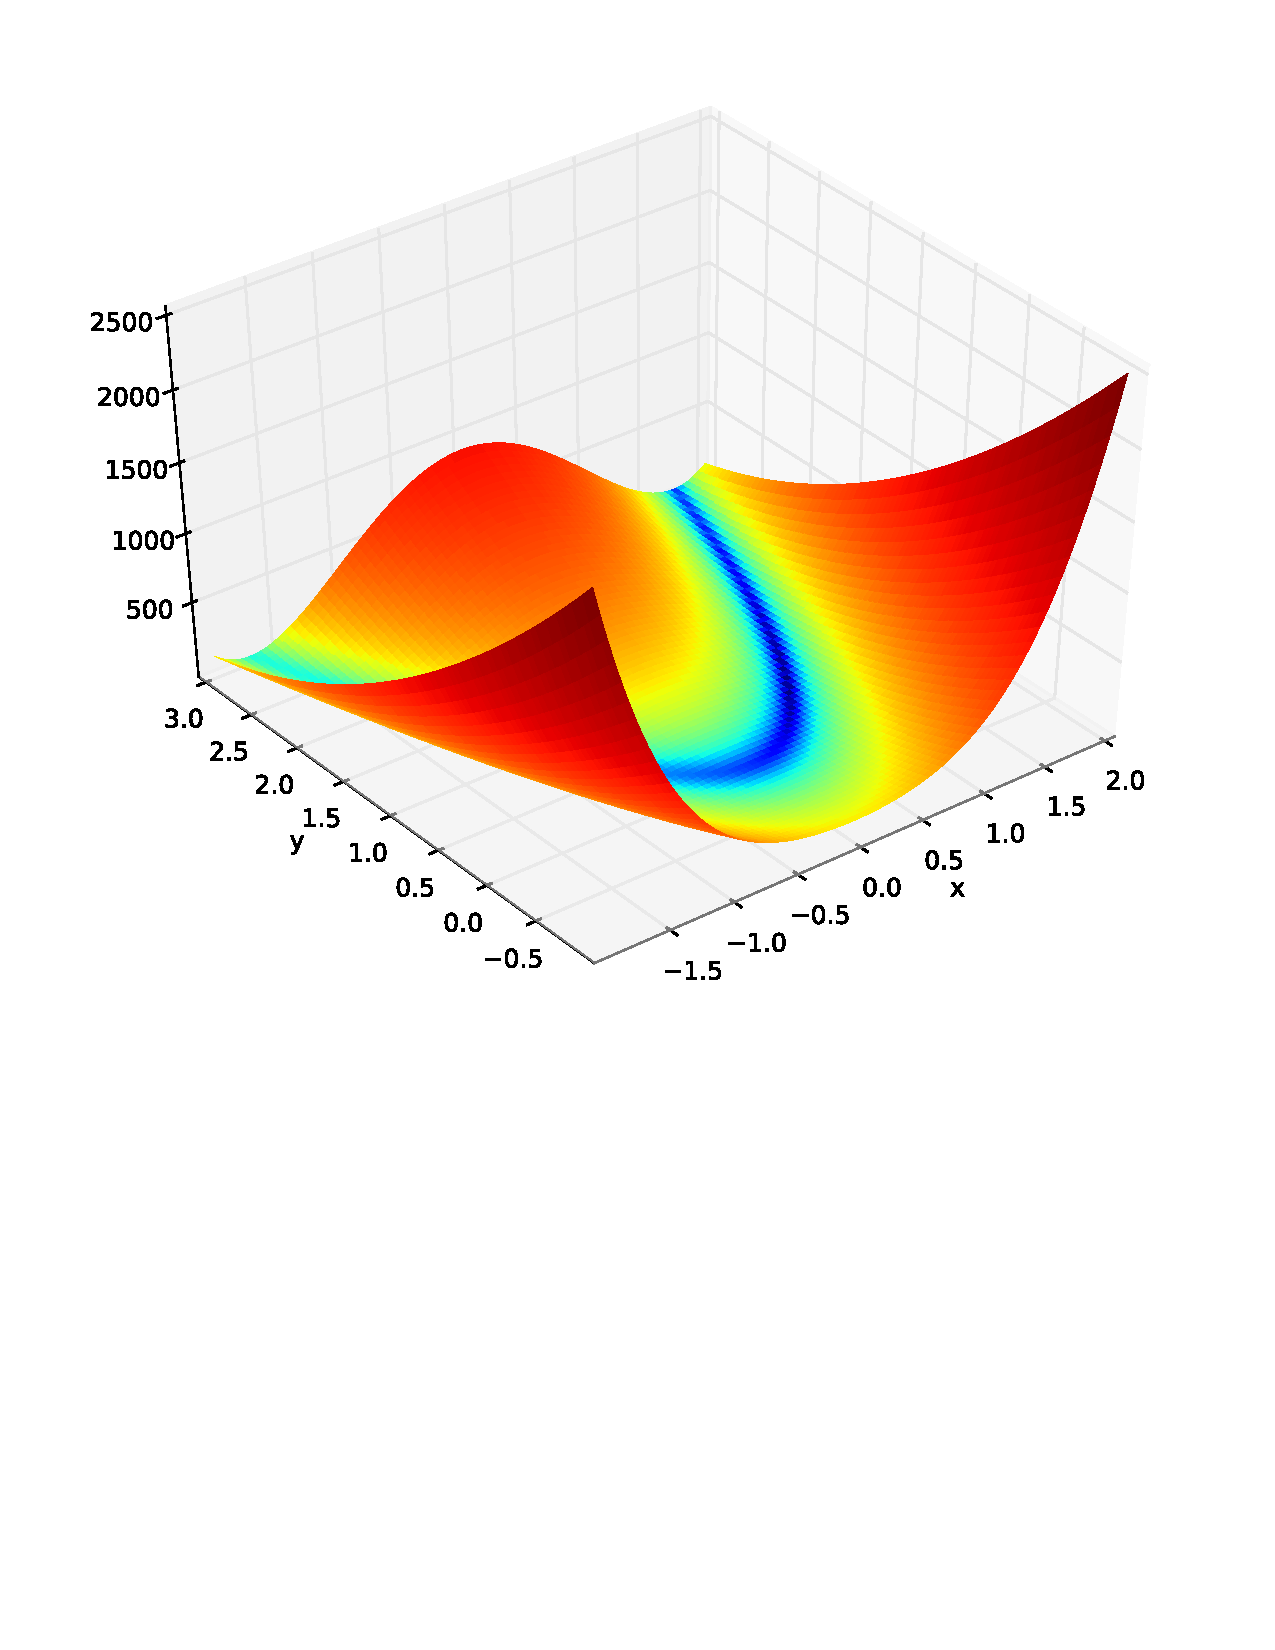
\includegraphics[width=.50\textwidth]{figs/rosenbrock}}
	\end{center}
	\caption{The Rosenbrock function. The global minimum is inside a long, narrow, parabolic shaped flat valley (Figure from \url{https://en.wikipedia.org/wiki/Rosenbrock_function})}
	\label{fig_rosenbrock}
\end{figure}

Its global minimum is at $(x,y) = (a,a^2)$, where $f(x,y)=0$. The parameters are usually set to $a=1$ and $b=100$, i.e.: 
\begin{align}
f(x,y) = (1-x)^2 + 100(y-x^2)^2.
\end{align}
With this choice of parameters, the minimum is at $(1,1)$. Indeed, this is the location of the minimum that is found by the following Python code using the {\tt scipy.optimize} library\footnote{\url{https://scipy-lectures.org/advanced/mathematical_optimization/}}: 

\begin{lstlisting}[language=Python]
def f(x):   # The Rosenbrock function
...     return (1.0 - x[0])**2 + 100.0*(x[1] - x[0]**2)**2
>>> optimize.minimize(f, [2, -1], method="CG")    
     fun: 1.6...e-11
     jac: array([-6.15...e-06,   2.53...e-07])
 message: ...'Optimization terminated successfully.'
    nfev: 108
     nit: 13
    njev: 27
  status: 0
 success: True
       x: array([0.99999...,  0.99998...])
\end{lstlisting}

To find the location of the minimum, the optimization function needs the derivatives (i.e., gradient, Jacobian). In the case of the Rosenbrock function from Equation \ref{rosenbrock}, the derivative (gradient in this case) is given by:
\begin{align}
\nabla f(x,y) = 
\begin{bmatrix}
-2(1-x) - 400\,y\,(y-x^2)\\
200(y - x^2)
\end{bmatrix}.
\end{align}
While the derivatives can be computed numerically by the library function, the optimization process is faster (and more accurate) if the user provides the analytical gradient to the Python optimization function. 

An example of passing the analytic derivative to the optimizer for finding the minimum of the Rosenbrock function is given by the following code:

\begin{lstlisting}[language=Python]
def jacobian(x):
        	Gx = -2.0*(1 - x[0]) - 400.0*x[0]*(x[1] - x[0]**2)
	Gy = 200.0*(x[1] - x[0]**2)       
...     return np.array((Gx,Gy))
>>> optimize.minimize(f, [2, 1], method="CG", jac=jacobian)    
     fun: 2.957...e-14
     jac: array([ 7.1825...e-07,  -2.9903...e-07])
 message: 'Optimization terminated successfully.'
    nfev: 16
     nit: 8
    njev: 16
  status: 0
 success: True
       x: array([1.0000...,  1.0000...])
\end{lstlisting}
When comparing the two optimization results, we can see that the second option is both more efficient (i.e., less function evaluations and less iterations) and more accurate (i.e., minimum was found at $[1,1]$ instead of at $[0.99999,0.99999]$) than the first option.\\

    \begin{mdframed}[backgroundcolor=green!20] 
        {\bf Summary}: Numerical-optimization methods produce faster and more precise results when we provide them with the analytical derivative (or gradient, or Jacobian) of the objective function. 
    \end{mdframed}

%% References 
\bibliographystyle{unsrt} 
\bibliography{refs}

\end{document}
% end of file template.tex




